\begin{frame}{Forklarbarhetsproblemet med kunstig intelligens}
    \begin{tikzpicture}
        \node[draw=black] at (-7, -3.25) {};
        \node[draw=black] at (7, 3.25) {};

        \only<1>{
            \inputside{-4.5}{-0.2175}{1.5cm}
            \cnnarrow{(input.east)}{($ (input.center) + (3, 0) $)}{black}
            \cnn{-2.7}{-0.2175}{0.1}{0.15}{uiogreen}{1}
            \node[anchor=west, align=left, font=\normalfont\linespread{0.9}\selectfont] (output1) at ($ (3.55, -0.2175) + (0, 0.5) $) {Pasient};
            \node[anchor=west, align=left, font=\normalfont\linespread{0.9}\selectfont] (output2) at ($ (3.55, -0.2175) - (0, 0.5) $) {Frisk\\kontroll};
            \cnnarrow{($ (output1.west) - (1, 0.5) $)}{($ (output1.west) + (0.1, 0) $)}{black}
            \cnnarrow{($ (output2.west) - (1, -0.5) $)}{($ (output2.west) + (0.1, 0) $)}{black}
        }
        \only<2-3>{
            \node[fill=gray!80, minimum width=4cm, minimum height=2.9cm, rounded corners=0.1cm, text=white, draw=black, font=\systemfont, anchor=south, text depth=2.4cm] (rule) at (0, 0) {
                Kunstig nevralt nettverk
            };
            \neuron{n00}{($ (rule.south) + (0, 1.25) + (-2*\hsep, -2*\vsep) $)}
            \neuron{n01}{($ (n00) + (0, \vsep) $)}
            \neuron{n02}{($ (n00) + (0, 2*\vsep) $)}
            \neuron{n03}{($ (n00) + (0, 3*\vsep) $)}
            \neuron{n04}{($ (n00) + (0, 4*\vsep) $)}

            \neuron{n10}{($ (n00) + (\hsep, 0.5*\vsep) $)}
            \neuron{n11}{($ (n00) + (\hsep, 1.5*\vsep) $)}
            \neuron{n12}{($ (n00) + (\hsep, 2.5*\vsep) $)}
            \neuron{n13}{($ (n00) + (\hsep, 3.5*\vsep) $)}

            \neuron{n20}{($ (n00) + (2*\hsep, \vsep) $)}
            \neuron{n21}{($ (n00) + (2*\hsep, 2*\vsep) $)}
            \neuron{n22}{($ (n00) + (2*\hsep, 3*\vsep) $)}

            \neuron{n30}{($ (n00) + (3*\hsep, 1.5*\vsep) $)}
            \neuron{n31}{($ (n00) + (3*\hsep, 2.5*\vsep) $)}

            \neuron{n40}{($ (n00) + (4*\hsep, 2*\vsep) $)}

            \foreach \j in {0,...,4} {
                \draw[black, opacity=\edgeopacity] ($ (rule.west) - (0, 0.2175) $) -- (n0\j);
            }

            \foreach \j in {0,...,4} {
                \foreach \k in {0,...,3} {
                    \draw[black, opacity=\edgeopacity] (n0\j) -- (n1\k);
                }
            }
            \foreach \j in {0,...,3} {
                \foreach \k in {0,...,2} {
                    \draw[black, opacity=\edgeopacity] (n1\j) -- (n2\k);
                }
            }
            \foreach \j in {0,...,2} {
                \foreach \k in {0,...,1} {
                    \draw[black, opacity=\edgeopacity] (n2\j) -- (n3\k);
                }
            }
            \draw[black, opacity=\edgeopacity] (n30) -- (n40);
            \draw[black, opacity=\edgeopacity] (n31) -- (n40);
            \draw[black, opacity=\edgeopacity] (n40) -- ($ (rule.south east) + (0, 1.25) $);

            \node[circle, draw=black, fill=uiogreen, minimum size=0.5cm] (neuron) at (0, -1.7) {};

            \node[anchor=east, font=\scriptsize] (x1) at ($ (neuron) - (0.75, -0.5) $) {$\text{input}_1$};
            \node[anchor=east, font=\scriptsize] (x2) at ($ (neuron) - (0.75, 0) $) {$\text{input}_2$};
            \node[anchor=east, font=\scriptsize] (x3) at ($ (neuron) - (0.75, 0.5) $) {$\text{input}_3$};

            \node[anchor=west, font=\scriptsize] (y) at ($ (neuron) + (0.75, 0) $) {$\text{output}$};

            \draw[-stealth] (x1) -- (neuron);
            \draw[-stealth] (x2) -- (neuron);
            \draw[-stealth] (x3) -- (neuron);
            \draw[-stealth] (neuron) -- (y);

            \node[font=\small] at ($ (neuron) + (0, 1) $) {
                Kunstig nevron
            };
        }
        \only<3>{
            \node[font=\small] at (0, -2.75) {
                $\text{output}=\text{max}(0, \text{input}_1*w_1+\text{input}_2*w_2+\text{input}_3*w_3)$
            };
        }

            % \node[anchor=east, inner sep=0pt, draw=black] (input) at (-3, 1.25) {
            %     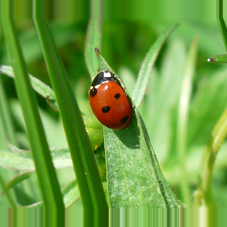
\includegraphics[width=2.5cm]{data/ladybug.png}
            % };
            % \node[anchor=west] (output) at (3, 1.25) {$\text{marihøne}$};

            % \draw[-stealth] (input) -- ($ (rule.south west) + (0, 1.25) $);
            % \draw[-stealth] ($ (rule.south east) + (0, 1.25) $) -- (output);
    \end{tikzpicture}
\end{frame}